\chapter{LaTeX testing stuff}
\label{LaTeX testing stuff}
{\color{red} 
{\huge Please ignore this chaper ...
This chapter will be excluded from final version.}
}

\begin{tikzpicture}[level distance=2cm,
level 1/.style={sibling distance=5.5cm},
level 2/.style={sibling distance=2.2cm},scale=1.2]
\node {\Large Puu test}
child {node {\large Siga}
child {node {esimene}}
}
child {node {\large Kala}
child {node {teine}}
child {node {kolmas}}
child {node {neljas}}
};
\end{tikzpicture}


{\huge\today}
\fontspec{Ubuntu}
Reason of this chapter is to test \LaTeX  stuff...
\rule{2.6cm}{0.75pt}  \hspace{3cm} üü \rule{3cm}{0.75pt}\\[2cm]
\begin{itemize}
	\item LaTeX testing stuff
	\item LaTeX testing stuff LaTeX testing stuff
\end{itemize}
\begin{Verbatim}[frame=single]
stuff
\end{Verbatim}

\ldots
\marginpar{\tiny This note will appear in the margin.}


\underline{Text you want underlined goes here.}


\begin{Verbatim}[frame=single,
label=Command output,framesep=2mm,rulecolor=\color{red},commandchars=\\\{\}]
margus@marguspc:~$ df -h
Filesystem             Size  Used Avail Use% Mounted on
/dev/sda1              239G  227G  6,0G  98% /
none                   4,0K     0  4,0K   0% /sys/fs/cgroup
udev                   3,9G  4,0K  3,9G   1% /dev
tmpfs                  790M  964K  789M   1% /run
none                   5,0M     0  5,0M   0% /run/lock
none                   3,9G   14M  3,9G   1% /run/shm
none                   100M   88K  100M   1% /run/user
/dev/sda1              239G  227G  6,0G  98% /home
\fbox{\color{red}/home/margus/.Private}  239G  227G  6,0G  98% /home/margus
\end{Verbatim}
%$

\section{Section name}
\begin{enumerate}
	\item Siia midagi nummerdatut
	\item veel midagi
\end{enumerate}
\subsection{subsection name}
Please see Figure ~\ref{Lab Setup} on page ~\pageref{Lab Setup} for bla bla bla.

\begin{minted}{c}
int main() {
printf("hello, world");
return 0;
}
\end{minted}
\begin{minted}{sh}
echo $(pidof mysql)
apt-get install firefox
$333
\end{minted}
\inputminted{sh}{code/simple.sh}

\begin{figure}
    \centering
	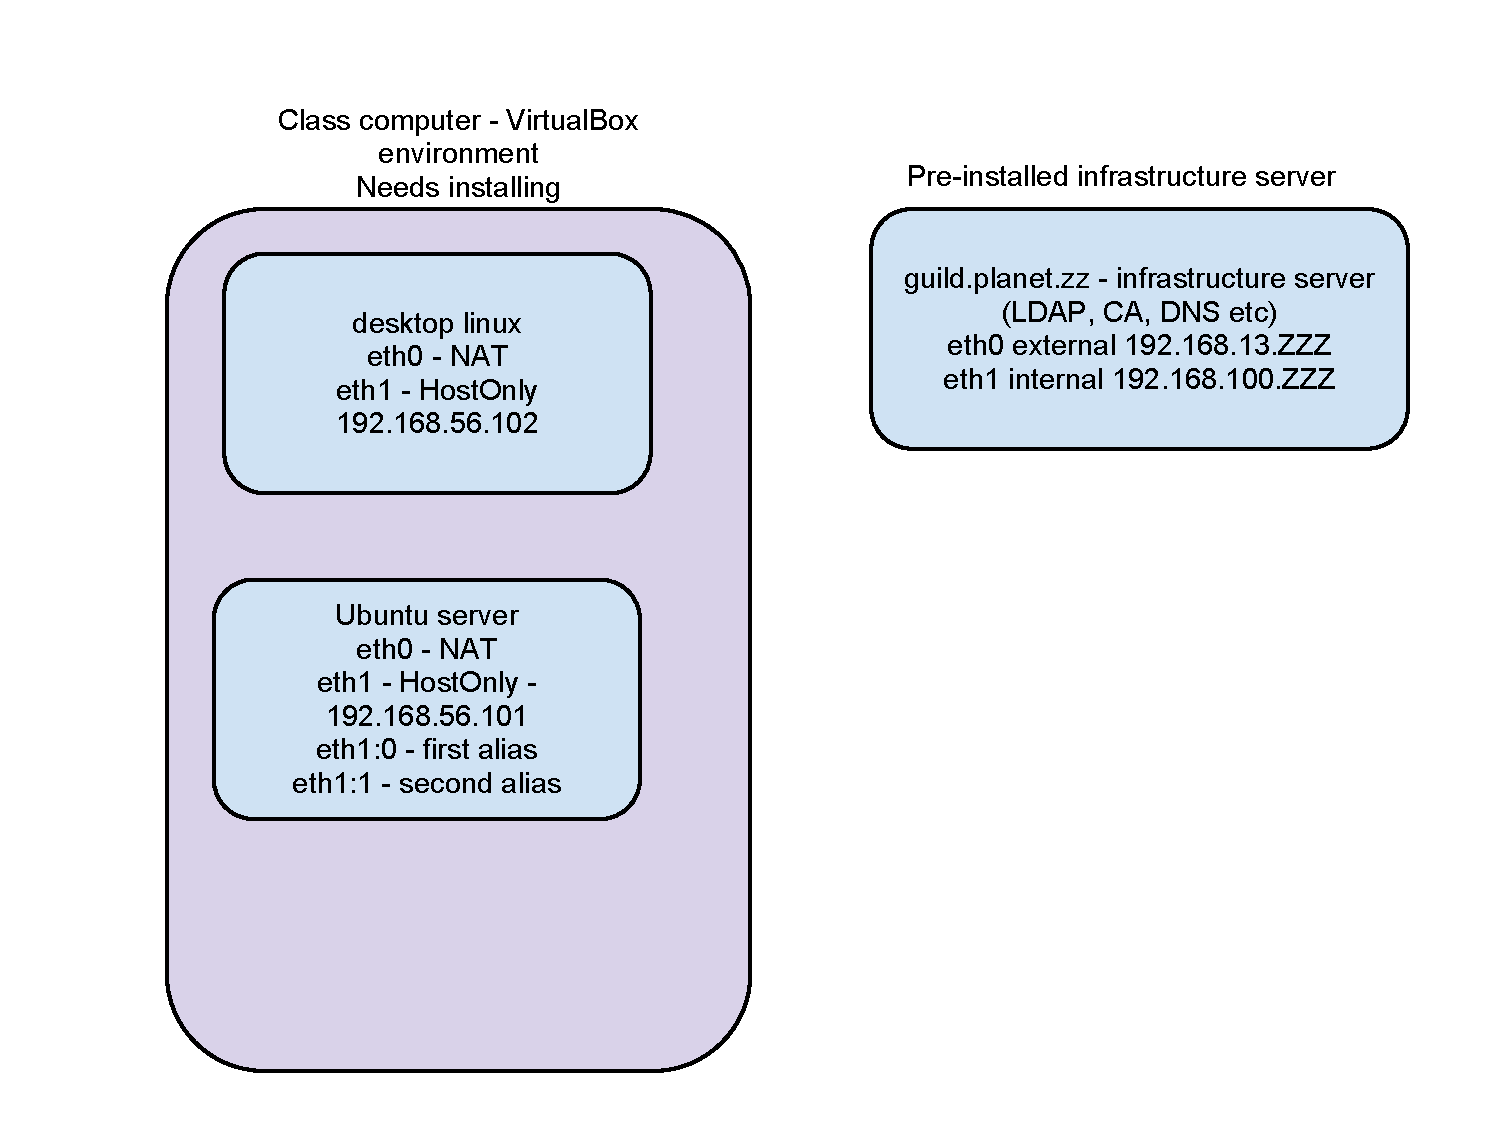
\includegraphics[width=\textwidth]{Lab_setup.pdf}
	\caption{Lab Setup}
	\label{Lab Setup}
\end{figure}


dddddd d  e d dwe \

\mint{ruby}|puts "hello world in ruby"|\

\cite{website:ssl} Bla bla
\citep{book:code-complete} d  d
\citep{OppeArenduskeskus2010} de dede
\cite{url:pulse} ewd wed
\citep{SecEngineering} wewde
The \gls{EITC} gives blaa blaa blaa.

Some unicode symbols
道場

\begin{tikzpicture}
  \path[mindmap,concept color=black,text=white]
    node[concept] {Computer Science}
    [clockwise from=0]
    child[concept color=green!50!black] {
      node[concept] {practical}
      [clockwise from=90]
      child { node[concept] {algorithms} }
      child { node[concept] {data structures} }
      child { node[concept] {pro\-gramming languages} }
      child { node[concept] {software engineer\-ing} }
    }  
    child[concept color=blue] {
      node[concept] {applied}
      [clockwise from=-30]
      child { node[concept] {databases} }
      child { node[concept] {WWW} }
    }
    child[concept color=red] { node[concept] {technical} }
    child[concept color=orange] { node[concept] {theoretical} };
\end{tikzpicture}

\begin{tikzpicture}
  \path[mindmap,concept color=black,text=white]
    node[concept] {Course pre requirements skills}
    [clockwise from=0]
    child[concept color=green!50!black] {
      node[concept] {GNU/Linux}
      [clockwise from=90]
      child { node[concept] {Able to use text editor} }
      child { node[concept] {Understanding of File System Hierarchy} }
      child { node[concept] {pro\-gramming languages} }
      child { node[concept] {software engineer\-ing} }
    }  
    child[concept color=blue] {
      node[concept] {Experience with command line}
      [clockwise from=-30]
      child { node[concept] {file manipulation with cp,mv,touch,rm,mkdir etc} }
      child { node[concept] {user management with adduser, passwd, id, getent, usermod, addgroup, useradd, groupadd} }
    }
    child[concept color=red] { node[concept] {technical} }
    child[concept color=orange] { node[concept] {theoretical} };
\end{tikzpicture}
